	\documentclass[10pt,oneside]{CBFT_book}
	% Algunos paquetes
	\usepackage{amssymb}
	\usepackage{amsmath}
	\usepackage{graphicx}
	\usepackage{libertine}
% 	\usepackage[bold-style=TeX]{unicode-math}
	\usepackage{lipsum}

	\usepackage{natbib}
	\setcitestyle{square}

	\usepackage{polyglossia}
	\setdefaultlanguage{spanish}


	\usepackage{CBFT.estilo} % Cargo la hoja de estilo

	% Tipografías
	% \setromanfont[Mapping=tex-text]{Linux Libertine O}
	% \setsansfont[Mapping=tex-text]{DejaVu Sans}
	% \setmonofont[Mapping=tex-text]{DejaVu Sans Mono}

	%===================================================================
	%	DOCUMENTO PROPIAMENTE DICHO
	%===================================================================

% \title{CBFT Mecánica clásica}
% \author{Cuerpos rígidos}
% \date{\today}

\begin{document}
% \maketitle
% \tableofcontents
\chapter{Cuerpos rígidos}

% =================================================================================================
\section{Cuerpos rígidos}
% =================================================================================================

Los vínculos constituyen la condición de rigidez,
\be
	|\vb{r}_i - \vb{r}_j | = d_{ij}	\qquad i \neq j
\label{vinculos}
\ee

Del discreto al continuo
\[
	\vb{R} = \frac{\sum_i m_i\vb{r}_i}{\sum_i m_i} \longrightarrow 
	\vb{R} = \frac{\int \rho \vb{r}_i dv }{\int \rho dv} 
\]

\subsection{Grados de libertad de un cuerpo rígido}

Cada punto tiene como vínculos las ecuaciones \eqref{vinculos}

\begin{figure}[htb]
	\begin{center}
	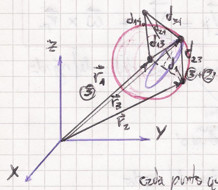
\includegraphics[width=0.45\textwidth]{images/fig_mc_rigidgl.pdf}	 
	\end{center}
	\caption{}
\end{figure} 

El cuerpo rígido tiene seis grados de libertad.
Si las condiciones de rigidez son lineales resultan cinco grados de libertad.

\subsection{Velocidad de un cuerpo rígido}

Lo único que pueden hacer los puntos de un cuerpo rígido es rotar.
\begin{figure}[htb]
	\begin{center}
	\includegraphics[width=0.35\textwidth]{images/fig_mc_rigidvel.pdf}	 
	\end{center}
	\caption{}
\end{figure} 
\[
	\delta r_{p_0} = r_{p_0} \sin(\beta) \delta \alpha
\]
\[
	\frac{\delta r_{p_0}}{\delta t} = r_{p_0} \sin(\beta) \frac{\delta\alpha}{\delta t}
\]
\[
	v_{p_0} = \dot{\alpha} r_{p_0} \sin(\beta)
\]
pero $v_{p_0} \perp \hat{n}$ y $v_{p_0} \perp r_{p_0}$ de manera que 
\[
	\vb{V}_{p_0} = \vb{\Omega} \times \vb{r}_{p_0}.
\]

Luego, para ir a un sistema inercial le sumo la V de algún punto del rígido (el origen O)
medido desde un sistema inercial. Entonces, el campo de velocidad del cuerpo rígido es
\[
	\vb{V}_{p} = \vb{V}_0 + \vb{\Omega} \times \vb{r}_{p_0}.
\]

\subsection{Unicidad de la velocidad de rotación}

\[
	\vb{V}_{p} = \vb{V}_0' + \vb{\Omega}' \times \vb{r}_{p_0'}
\]
siendo \vb{\Omega}' la \vb{\Omega} como se ve desde el sistema O'
\[
	\vb{V}_{p} = \vb{V}_0 + \vb{\Omega} \times \vb{r}_{p_0}
\]
y donde \vb{\Omega} es la vista desde el sistema O.
\begin{figure}[htb]
	\begin{center}
	\includegraphics[width=0.35\textwidth]{images/fig_mc_velrot.pdf}	 
	\end{center}
	\caption{}
\end{figure} 
\[
	\vb{V}_0' + \vb{\Omega}' \times \vb{r}_{p_0'} = \vb{V}_0 + \vb{\Omega} \times \vb{r}_{p_0} 
\]
y descomponiendo de acuerdo con el dibujo resulta 
\[
	\vb{\Omega} \times \vb{r}_{OO'} + \vb{\Omega}' \times \vb{r}_{0'p} = \vb{\Omega} \times \vb{r}_{p_0} 
\]
\[
	\vb{\Omega} \times ( \vb{r}_{00'} - \vb{r}_{0p} ) + \vb{\Omega}' \times \vb{r}_{0'p}  = 0
\]
\[
	( \vb{\Omega}' - \vb{\Omega}  ) \times \vb{r}_{0'p} = 0 ,
\]
de la cual se deduce que $\vb{\Omega}'=\vb{\Omega}$. Entonces, \vb{\Omega} es la misma para cualquier
punto del cuerpo rígido.

\[
	\vb{\Omega} \cdot \vb{V}_p = \vb{\Omega} \cdot \vb{V}_0  + \vb{\Omega}\cdot(\vb{\Omega}\times \vb{r}_{0p} )
\]
\[
	\vb{\Omega} \cdot \vb{V}_p = \vb{\Omega} \cdot \vb{V}_0
\]
lo cual se cumple para todo punto $p$ perteneciente al cuerpo rigido. Si es $\vb{\Omega} \cdot \vb{V}_0 = 0$
entonces serán $\vb{\Omega} \perp \vb{V}_0$ y $\vb{\Omega} \perp \vb{V}_p$.

Si en un instante dado \vb{\Omega} es perpendicular a $\vb{V}_p$ entonces \vb{\Omega} es perpendicular a 
$\vb{V}_{p'}$ para todo punto del cuerpo rígido.

\subsection{Eje instantáneo de rotación}

Si $p$ es tal que $\vb{V}_p = 0$ entonces
\[
	\vb{V}_0 = - \vb{\Omega} \times \vb{r}_{p0}
\]
donde $\vb{V}_0$ es una velocidad desde un sistema inercial.
Desde el sistema inercial el cuerpo rígido realiza una rotación pura, puesto que veo al
punto O rotar en torno a algún eje.
\[
	\vb{V}_0 = - \vb{\Omega} \times ( r_{\perp} + r_{\parallel} ) = -\vb{\Omega} \times  r_{\perp} 
\]
y esto define un eje instantáneo de rotación.
\begin{figure}[htb]
	\begin{center}
	\includegraphics[width=0.5\textwidth]{images/fig_mc_ejeinst.pdf}	 
	\end{center}
	\caption{}
\end{figure} 

% =================================================================================================
\section{Ángulos de Euler}
% =================================================================================================

Se toma un sistema 123 inicialmente coincidente con uno XYZ paralelo al inercial, 123 tiene origen
en el centro de masa del cuerpo.
\begin{figure}[htb]
	\begin{center}
	\includegraphics[width=0.5\textwidth]{images/fig_mc_eulerangles.pdf}	 
	\end{center}
	\caption{}
\end{figure} 
\[
	A_1(\phi) = 
	\begin{pmatrix}
		\cos(\phi) & \sin(\phi) & 0 \\
		-\sin(\phi) & \cos(\phi) & 0 \\ 
		0 & 0 & 1  \\
	\end{pmatrix}
\]
\[
	A_2(\theta) = 
	\begin{pmatrix}
		1 & 0 & 0 \\
		0 & \cos(\theta) & \sin(\theta) \\ 
		0 & -\sin(\theta) & \cos(\theta)  \\
	\end{pmatrix}
\]
\[
	A_3(\psi) = 
	\begin{pmatrix}
		\cos(\psi) & \sin(\psi) & 0 \\
		-\sin(\psi) & \cos(\psi) & 0 \\ 
		0 & 0 & 1  \\
	\end{pmatrix}
\]
\[
	\vb{\Omega} = \dot{\phi}\hat{z} + \dot{\theta}\hat{n} + \dot{\psi}\hat{3}
\]
y expresando $\hat{z},\hat{n}$ en $\hat{1},\hat{2}, \hat{3}$ resulta
\[
	\vb{\Omega} = [\dot{\phi}\sin(\theta)\sin(\psi) + \dot{\theta}\cos(\psi) ]\hat{1} +
			[\dot{\phi}\sin(\theta)\cos(\psi) - \dot{\theta}\sin(\psi) ] \hat{2} +
			[\dot{\phi}\cos(\theta) + \dot{\psi} ]\hat{3}
\]

Ahora estamos interesados en el momento angular.
\[
	\vb{L}_0^{sist} = \vb{L}^{cm} + \vb{L}_{cm}^{sist} 
\]
\[
	\vb{L}_{spin} = \sum_i^N m_i ( \vb{r}_i' \times \vb{v}_i' )
\]
que están en el sistema 123.
\[
	\vb{L}_{spin} = \sum_i^N m_i ( \vb{r}_i \times \vb{\Omega} \times \vb{r}_i )
\]
\[
	\vb{L}_{spin} = \sum_i^N m_i \left[ \; 
	\vb{\Omega} (\vb{r}_i\cdot\vb{r}_i) - \vb{r}_i(\vb{r}_i \cdot \vb{\Omega}) \; \right] 
\]
\[
	\vb{L}_{spin} = \sum_i^N m_i \left[ \; 
	\vb{\Omega} \sum_j^3 (x_j^{2i}) - \vb{r}_i \sum_\ell^3 x_\ell^i \Omega_\ell  \; \right] 
\]
y la componente $k$-ésima será 
\[
	L_k = \sum_i^N m_i \left[ \; 
	\Omega_k \sum_j^3 (x_j^{2i}) - x_k^i \sum_\ell^3 x_\ell^i \Omega_\ell  \; \right] 
\]
\[
	L_k = \sum_i^N m_i \left[ \; 
	\sum_j^3 \delta_{kj} \Omega_j r_i^{2} - x_k^i \sum_\ell^3 x_\ell^i \Omega_\ell  \; \right] 
\]
\[
	L_k = \sum_j^3 \sum_i^N m_i \left[ \; 
	\delta_{kj} r_i^{2} - x_k^i x_j^i  \; \right] \Omega_j = \sum_j^3 I_{kj} \Omega_j 
\]
o vectorialmente
\[
	\vb{L}_{spin} = I \vb{\Omega}
\]
siendo $I$ el tensor de inercia. Explícitamente:
\[
	I_{kj} = \sum_i^N m_i \left[ \; \delta_{kj} r_i^{2} - x_k^i x_j^i  \; \right]
\]
\[
	\begin{pmatrix}
		L_1 \\
		L_2 \\ 
		L_3  \\
	\end{pmatrix} 
	=
	\begin{pmatrix}
		I_{11} & I_{12} & I_{13} \\
		I_{21} & I_{22} & I_{23} \\ 
		I_{31} & I_{32} & I_{33}  \\
	\end{pmatrix}
	\begin{pmatrix}
		\Omega_1 \\
		\Omega_2 \\ 
		\Omega_3  \\
	\end{pmatrix} 
\]

Sean 1,2,3 los ejes principales, entonces $I$ es diagonal y
\[
	\vb{L}_{spin}
	=
	\begin{pmatrix}
		I_{11} & 0 & 0 \\
		0 & I_{22} & 0 \\ 
		0 & 0 & I_{33}  \\
	\end{pmatrix}
	\begin{pmatrix}
		\Omega_1 \\
		\Omega_2 \\ 
		\Omega_3  \\
	\end{pmatrix}
	=
	I \vb{\Omega}
\]
y se puede escribir
\[
	\left.\frac{d}{dt}\right|_{in} \Box = \left.\frac{d}{dt}\right|_{rot} \Box + \vb{\Omega} \times \Box
\]
que es válida pra sistemas rotantes (no aquellos que rotan y se trasladan).
En este caso \vb{\Omega} es la del sistema rotante (en un cuerpo rígido es la \vb{\Omega} del cuerpo rígido).

Se puede escribir también 
\[
	\left.\frac{d}{dt}\right|_{in} \vb{L}_{spin} = \vb{\Tau}_{cm}
\]
siendo la derivada de uns sitema XYZ, y \vb{\Tau} el torque del cuerpo rígido referido al centro de masa y
medido dese el sistema XYZ (inercial).
Entonces
\[
	\vb{\Tau}_{cm} = \left. \frac{d}{dt}\right|_{rot} \vb{L}_{spin} + \vb{\Omega} \times ( \vb{L}_{spin} )
\]
y
\[
	\vb{\Tau}_{cm} = \left. I \frac{d}{dt}\right|_{rot} \vb{\Omega} + \vb{\Omega} \times ( I \; \vb{\Omega} ).
\]
$I$ visto desde XYZ es $I=I(t)$ e $I$ desde 123 es constante.
\[
	\vb{\Tau}_{cm} =
	\begin{pmatrix} \;
		I_1 \dot{\vb{\Omega}}_1 \\
		I_2 \dot{\vb{\Omega}}_2 \\ 
		I_3 \dot{\vb{\Omega}}_3 \; \\
	\end{pmatrix}
	+
	\begin{vmatrix} \;
		\hat{1} & \hat{2} & \hat{3} \\
		\; \Omega_1 & \Omega_2 & \Omega_3 \\ 
		\; I_1\Omega_1 & I_2\Omega_2 & I_3\Omega_3 \; \\
	\end{vmatrix}	
\]

De este sistema resultan,
\begin{align*}
\Tau_1 = I_1 \dot{\Omega}_1 + (I_3-I_2) \: \Omega_2 \: \Omega_3 \\
\Tau_2 = I_2 \dot{\Omega}_2 + (I_1-I_3) \: \Omega_3 \: \Omega_1 \\
\Tau_3 = I_3 \dot{\Omega}_3 + (I_2-I_1) \: \Omega_1 \: \Omega_2
\end{align*}
que son las ecuaciones de Euler. 
Las mismas requieren $I$ en ejes principales, \vb{\Omega} en 1,2,3 (en función de $\phi,\theta,\psi$).
Es \vb{\Omega} la velocidad de rotación del sistema cuerpo rígido (rotante) respecto a un sistema XYZ
fijo en el centro de masa y coincidente con X'Y'Z' (inercial) a todo tiempo. Salvo la traslación del centro
de masa, este sistema XYZ será inercial.

Todo este tratamiento de ecuaciones de Euler es para el caso $\vb{L}_{spin} \equiv \vb{L}_{cm}^{sist}$, de
manera que no me importan las traslaciones del centro de masa.

\[
	\left.\frac{d}{dt}\right|_{XYZ} \vb{L}_{spin} = \vb{\Tau}_{cm} =
	\left.\frac{d}{dt}\right|_{123} \vb{L}_{spin} + \vb{\Omega} \times \vb{L}_{spin} 
\]

% =================================================================================================
\section{Energía cinética del cuerpo rígido}
% =================================================================================================

Queremos escribir la energía cinética de un cuerpo rígido explícitamente en términos del momento
de inercia $I$.
\[
	T = \frac{1}{2} \sum_i^N m_i v_i^2 = \frac{1}{2} \sum_i^N m_i ( \vb{v}_{cm} + \vb{\Omega} \times \vb{r}_i ) ^2
\]
donde la última $\vb{r}_i$ está referida al centro de masa (posiciones de los puntos del cuerpo
rígido referidas al centro de masa).
\[
	T = \frac{1}{2} \sum_i^N m_i ( \vb{v}_{cm}^2 + (\vb{\Omega} \times \vb{r}_i)^2 +
		2 \vb{v}_{cm} \cdot (\vb{\Omega} \times \vb{r}_i)  )
\]
pero es fácil ver que el término de cruza es cero dado que 
\[
	\sum_i^N m_i \vb{v}_{cm} \cdot (\vb{\Omega} \times \vb{r}_i) = 
	\sum_i^N m_i \vb{r}_i \cdot ( \vb{v}_{cm} \times \vb{\Omega} ) = 
	M \vb{R}_{cm} \cdot ( \vb{v}_{cm} \times \vb{\Omega} ) = 0
\]
puesto que $M \vb{R}_{cm}$ es nulo para un sistema no inercial. Luego 
\[
	T = \frac{1}{2} \sum_i^N m_i \vb{v}_{cm}^2 + \frac{1}{2} \sum_i^N m_i (\vb{\Omega} \times \vb{r}_i)^2
\]
\[
	T = \frac{1}{2} \sum_i^N m_i \vb{v}_{cm}^2 +
	\frac{1}{2} \sum_i^N m_i ( \Omega^2 r_i^2 - (\vb{\Omega}\cdot\vb{r}_i)^2 )
\]
pero veamos el último paréntesis en detalle,
\[
	\left(\sum_j \sum_k \Omega_j \Omega_j x_k^i x_k^i - 
	\sum_\ell \sum_p \Omega_\ell x_\ell^i \Omega_p x_p^i \right)
\]
\[
	\left(\sum_j \sum_k \Omega_j \delta_{jk}\Omega_k x_k^i x_k^i - 
	\sum_\ell \sum_p \Omega_\ell x_\ell^i \Omega_p x_p^i \right)
\]
y reetiquetando
\[
	\left(\sum_j \sum_k \Omega_j \delta_{jk}\Omega_k x_k^i x_k^i - 
	\sum_j \sum_k \Omega_j x_j^i \Omega_p x_k^i \right)
\]
\[
	\frac{1}{2} \sum_i^N m_i \sum_{j,k} \Omega_j\Omega_k \left[ \delta_{jk}(r^i)^2 - x^i_j x^i_k \right]
\]
y entonces
\[
	T = \frac{1}{2} M V^2_{cm} + \frac{1}{2} \sum_{j,k} \Omega_j\Omega_k I_{jk}
\]
y como lo último es una forma cuadrática podemos escribir de manera más elegante
\[
	T = \frac{1}{2} M V^2_{cm} + \frac{1}{2} \vb{\Omega}^t I \vb{\Omega}. 
\]

Recordemos que el tensor de inercia tiene en su diagonal los momentos de inercia
mientras que los términos fuera de la misma son los productos de inercia.
\[
	I_{ik} = \sum_q m_q \left( \delta_{ik} (r_q)^2 - x_i^q x_k^q \right)
\]
y el paso al continuo nos deja los momentos de inercia,
\[
	I_{ik} = \int_V \rho(\vb{r}) \left[ \delta_{ik}r^2 - x_i x_k \right] dV
\]
donde por supuesto es $r^2 = x_1^2 + x_2^2 + x_3^2$.

El cambio de sistema se hace de acuerdo a
\[
	I_{ik}' = \sum_{\ell s} a_{i\ell} I_{\ell s} a_{ks}
\]
y en componentes,
\[
	\sum_q m_q ( \delta_{ik} {r'}^2_q - x'_i x'_k ) =  a_{i\ell} a_{ks} \sum_q m_q
	( \delta_{\ell s} r^2_q - x_\ell x_s )
\]
donde en el miembro izquierdo es $i \neq k$, y el derecho $\ell \neq s$
\[
	- \sum_q m_q x'_i x'_k =  - \sum_q m_q a_{i\ell} x_\ell a_{ks}  x_s 
\]
entonces 
\[
	I =
	\begin{pmatrix} \;
		I_{11} & I_{12} & I_{13} \\
		I_{21} & I_{22} & I_{23} \\ 
		I_{31} & I_{32} & I_{33} \\
	\end{pmatrix}
\]
siendo el triángulo superior valores repetidos. El tensor de inercia es simétrico por su 
definición. De los nueve componentes son independientes seis. Matemáticamente
\[
	I_{ik} = I_{ki}.
\]

Todo tensor simétrico se puede llevar a una forma diagonal eligiendo bien los ejes del 
sistema 123 fijo al cuerpo. Podemos conseguir una transformación $I \to I'$ tal que 
\[
	I' =
	\begin{pmatrix} \;
		I_{11}' & 0 & 0 \\
		0 & I_{22}' & 0 \\ 
		0 & 0 & I_{33}' \\
	\end{pmatrix}
\]
Los $I'_{ik}$ son los momentos principales de inercia (aquellos que están calculados sobre
{\it ejes principales de inercia}).

Cuando el cuerpo rígido tiene simetría pueden hallarse a ojo los ejes principales de inercia.

Para el cálculo de $I$ se usa un sistema fijo al cuerpo rígido. Si usamos un sistema inercial,
será $I_{ik}=I_{ik}(t)$ lo cual no es conveniente.

Es conveniente elegir 123 con origen en el centro de masa y partícipes del movimiento del 
cuerpo rígido (clavados al mismo). Asimismo conviene elegir XYZ referidos al sistema inercial
coincidentes pero trasladados al centro de masa. Así los $I_{ik}$ resultan características
geométricas del cuerpo.

% =================================================================================================
\section{La peonza simétrica}
% =================================================================================================

\[
	T_{rot} = \frac{1}{2} I_1 \Omega^2_ 1 + \frac{1}{2} I_2 \Omega^2_2 + \frac{1}{2} I_3 \Omega^2_3 
\]
donde son 
\[
	\Omega_1 = \dot{\theta} \qquad \Omega_2 = \dot{\phi} \sin(\theta) \qquad \Omega_3 = \dot{\phi} \cos(\theta) + \dot{\psi}
\]
y debemos destacar que $\psi=0$ no es vínculo sino solo comodidad pues $\dot{\psi} \neq 0$ y es independiente.
Los vínculos pueden escribirse
\[
	\theta_e = \theta
\]
\[
	\phi_e + \frac{3}{2}\pi = \phi \; \longrightarrow \; \dot{\phi_e} = \dot{\phi}
\]
\[
	r^2 = a^2 = x_{cm}^2 + y_{cm}^2 + z_{cm}^2
\]
\begin{figure}[htb]
	\begin{center}
	\includegraphics[width=0.5\textwidth]{images/fig_mc_peonza1.pdf}	 
	\end{center}
	\caption{}
\end{figure} 
y las coordenadas
\begin{align*}
	x &= a \sin(\theta) \cos\left( \frac{\pi}{2}-\phi_e \right) = a \sin(\theta) \sin( \phi_e ) \\
	y &= a \sin(\theta) \sin\left( \frac{\pi}{2}-\phi_e \right) = -a \sin(\theta) \cos( \phi_e ) \\
	z &= a \cos(\theta)
\end{align*}
y la velocidad
\[
	\dot{x}^2 + \dot{y}^2 + \dot{z}^2 = a^2 \dot{\theta}^2 + a^2 \sin(\theta)^2 \dot{\phi}^2
\]
y el lagrangiano finalmente
\[
	\Lag = \frac{1}{2} M (a^2 \dot{\theta}^2 + a^2 \sin(\theta)^2 \dot{\phi}^2) + \frac{1}{2} I_1 \dot{\theta}^2
	+ \frac{1}{2} I_2 \sin(\theta)^2 \dot{\phi}^2) + \frac{1}{2} I_3 (\dot{\phi} \cos(\theta) + \dot{\psi})^2 
\]
pero por la simetría $I_1=I_2\equiv I$ de modo que 
\[
	\Lag = \frac{1}{2} M a^2 (\dot{\theta}^2 + \sin(\theta)^2 \dot{\phi}^2) + \frac{1}{2} I ( \dot{\theta}^2 +
	\sin(\theta)^2 \dot{\phi}^2 ) + \frac{1}{2} I_3 (\dot{\phi} \cos(\theta) + \dot{\psi})^2 
\]
\[
	\Lag = \frac{1}{2} ( M a^2 + I ) (\dot{\theta}^2 + \sin(\theta)^2 \dot{\phi}^2) +  
		\frac{1}{2} I_3 (\dot{\phi} \cos(\theta) + \dot{\psi})^2  - m g a \cos(\theta)
\]
y los primeros dos términos representan una rotación pura si tomo 
\[
	( M a^2 + I ) \equiv I' 
\]
donde $I'$ es otro momento de inercia.
\begin{figure}[htb]
	\begin{center}
	\includegraphics[width=0.5\textwidth]{images/fig_mc_peonza2.pdf}	 
	\end{center}
	\caption{}
\end{figure} 

Luego hay unos interesantes comentarios sobre la ubicación de los ejes. El famoso ``bajo ejes''.
\[
	T = T_{trasl} + T_{rot} + T_{acopl}
\]
y el último es nulo si elegimos el origen común O=O'= centro de masa.
\[
	\vb{V} = \vb{V}_{cm} + \Omega \times \vb{r}
\]
También es $T_{acopl}=0$ si $V_0=0$ (aquí también se anula $T_{trasl}$).

% =================================================================================================
\section{Teorema de Steiner}
% =================================================================================================

\[
	\vb{x} = \vb{U} - \vb{a}  
\]
\[
	I_{ij}^0 = \sum_s^N m^s ( \delta_{ij} x_s^2 - x_i^s x_j^s )
\]
\[
	I_{ij}^0 = \sum_s^N m^s ( \delta_{ij} ( \vb{U}_s - \vb{a} )^2 - (U^s_i - a_i) ( U^s_j - a_j ) )
\]
\begin{figure}[htb]
	\begin{center}
	\includegraphics[width=0.5\textwidth]{images/fig_mc_steiner1.pdf}	 
	\end{center}
	\caption{}
\end{figure} 
Trasladamos el punto (con el sistema de ejes paralelo al del centro de masa) sin rotarlo. Eso es importante.
\[
	I_{ij}^0 = \sum_s^N m^s \left[  \delta_{ij} ( U_s^2 + a^2 - 2Ua ) -
			( U^s_iU^s_j + a_i a_j - a_i U^s_j - a_j U^s_i ) \right]
\]
\[
	I_{ij}^0 = \sum_s^N m^s ( \delta_{ij} U_s^2 - U^s_iU^s_j ) + \sum_s^N m^s ( \delta_{ij} a^2 - a_i a_j )
			- \sum_s^N m^s \delta_{ij} 2 U^s a  + \sum_s^N m^s ( a_i U^s_j + a_j U^s_i )
\]
pero las dos últimas sumatorias son nulas, y
\[
	I_{ij}^0 = \sum_s^N m^s ( \delta_{ij} U_s^2 - U^s_iU^s_j ) + \sum_s^N m^s ( \delta_{ij} a^2 - a_i a_j )
		= I_{ij}^{cm}  + M ( \delta_{ij} a^2 - a_i a_j )
\]

Esto sale de
\[
	\sum_s^N m^s \delta_{ij} U^s a = \delta_{ij} a \sum_s^N m^s  U^s  = 0
\]
puesto que es nula la suma en $s$. Porque 
\[
	0 = \sum_s^N m^s \vb{U}^s = \sum_s^N m^s ( U_1^s \hat{1} + U_2^s \hat{2} + U_3^s \hat{3} )
\]
pero como es vectorial vale para cada coordenada 
\[
	0 = \sum_s^N m^s U_i^s \qquad \forall i=1,2,3
\]
\[
	0 = \sum_s^N m^s U_i^s a
\]
\begin{figure}
	\begin{center}
	\includegraphics[width=0.5\textwidth]{images/fig_mc_steiner2.pdf}	 
	\end{center}
	\caption{}
\end{figure} 
La moraleja es que trasladar en un solo eje conserva la diagonalidad del tensor de inercia.

% =================================================================================================
\section{Sistemas no inerciales}
% =================================================================================================

\begin{figure}
	\begin{center}
	\includegraphics[width=0.7\textwidth]{images/fig_sist_rotantes.pdf}	 
	\end{center}
	\caption{Sistemas rotantes.}
\end{figure} 

\vb{\Omega} es la velocidad angular del sistema no inercial. $\ddot{\vb{R}}$ es la aceleración del 
sistema no inercial. Ambas se miden sólo desde el sistema inercial.

\[
	\vb{r} = \vb{R} + \vb{r}'
\]
\[
	\left.\dtot{\vb{r}}{t}\right|_{in} =
			\left.\dtot{\vb{R}}{t}\right|_{in} + \left.\dtot{\vb{r}'}{t}\right|_{in}
\]
si despejamos la derivada respecto del sistema primado,
\[
	\left.\dtot{\vb{r}'}{t}\right|_{in} = \left.\dtot{\vb{r}}{t}\right|_{in} 
				- \left.\dtot{\vb{R}}{t}\right|_{in}
\]
y usamos 
\[
	\left.\dtot{\vb{r}'}{t}\right|_{in} = \left.\dtot{\vb{r}'}{t}\right|_{no in} +
				\vb{\Omega} \times \vb{r}'
\]
va resultando 
\[
	\left. \frac{d}{dt}\left( {\left.\dtot{\vb{r}'}{t}\right|_{no in}} \right) \right|_{in}  =  
			\left.\dtot[2]{\vb{r}}{t}\right|_{in}  - \left.\dtot[2]{\vb{R}}{t}\right|_{in} 
			- \left. \dtot{(\vb{\Omega} \times \vb{r}')}{t}\right|_{in}
\]
\[
	\left.\dtot[2]{\vb{r}'}{t}\right|_{no in}  + \vb{\Omega} \times \left.\dtot{\vb{r}'}{t}\right|_{no in}
		 = \vb{a}|_{in} - \ddot{\vb{R}}|_{in} - \left. \dtot{\vb{\Omega}}{t}\right|_{in} \times \vb{r}' 
				+ \vb{\Omega} \times \left. \dtot{ \vb{r}'}{t}\right|_{in}
\]
donde hemos usado que 
\[
	\left. \dtot{\vb{\Omega}}{t} \right|_{in} = \left. \dtot{\vb{\Omega}}{t} \right|_{no in} \qquad \qquad
	\left. \dtot{\vb{R}}{t} \right|_{in} = - \left. \dtot{\vb{R}}{t} \right|_{no in}
\]
\[
	\left.\dtot[2]{\vb{r}'}{t}\right|_{no in}  + \left( \vb{\Omega} \times \left.\dtot{\vb{r}'}{t}\right|_{no in} \right)
		 = \vb{a}|_{in} - \ddot{\vb{R}}|_{in} 
		 - \left[\left. \dtot{\vb{\Omega}}{t}\right|_{no in} + \vb{\Omega} \times \vb{\Omega} \right] \times \vb{r}' 
		+ \vb{\Omega} \times \left[ \left. \dtot{ \vb{r}'}{t}\right|_{no in} + \vb{\Omega} \times \vb{r}' \right]
\]
\[
	\left. \vb{a}'\right|_{no in}   = \vb{a}|_{in} - \ddot{\vb{R}}|_{in} 
		 - \dot{\vb{\Omega}} \times \vb{r}'  -  \vb{\Omega} \times \left.\dot{\vb{r}}' \right|_{no in} 
		- \vb{\Omega} \times \left( \vb{\Omega} \times \dot{\vb{r}}' \right) 
		- \vb{\Omega} \times  \left. \dtot{ \vb{r}'}{t}\right|_{no in} 
\]
\[
	\left. \vb{a}'\right|_{no in}  = \ddot{\vb{r}}  - \ddot{\vb{R}}
		 - \dot{\vb{\Omega}} \times \vb{r}'  -  2 \vb{\Omega} \times \left.\dot{\vb{r}}' \right|_{no in} 
		- \vb{\Omega} \times \left( \vb{\Omega} \times \dot{\vb{r}}' \right)
\]

Vale la pena aclarar la deduccion,
\[
	\left. \dtot{\vb{r}}{t} \right|_{in} = \left. \dtot{\vb{R}}{t} \right|_{in} + \left. \dtot{\vb{r}'}{t} \right|_{no in}
	+ \vb{\Omega} \times \vb{r}' 
\]
pero si es $\vb{R}=0$ se tiene $\vb{r}=\vb{r}'$ y entonces
\[
	\left. \dtot{\vb{r}}{t} \right|_{in} =  \left. \dtot{\vb{r}'}{t} \right|_{no in} + \vb{\Omega} \times \vb{r}' 
\]
donde el sistema no inercial es el rotante.

% =================================================================================================
\section{Lagrangiano de un sistema no inercial que se traslada}
% =================================================================================================

\[
	\Lag = \frac{1}{2} m v^2 - U(\vb{r})
\]
\[
	\Lag = \frac{1}{2} m ( v + v' )^2 - U(\vb{r})
\]
\[
	\Lag = \frac{1}{2} m  v^2 + m \vb{v}\cdot\vb{v}' +\frac{1}{2} m {v'}^2 - U(\vb{r}) - U
\]
pero el primer término se  tira puesto que equivale a un término $df/dt$ que cumple 
\[
	\dtot{f}{t} = \frac{1}{2} m  v^2 \qquad \qquad f = \frac{1}{2} m  \frac{v^3}{3} + K
\]
y además 
\[
	 m \vb{v}\cdot\vb{v}' =  m \vb{v}\cdot \dtot{\vb{v}'}{t} = - m \dtot{\vb{v}}{t} \vb{r}' 
				+ \frac{d}{dt}\left( m \vb{r}' \vb{v} \right)
\]
y el último término acá lo tiramos porque equivale a un $df_2/dt$.
\[
	\Lag = \frac{1}{2} m {v'}^2 - m \dtot{\vb{v}}{t}\cdot\vb{r}' - U(\vb{r})
\]
\[
	\dtot{\dpar{\Lag}{\vb{v}'}}{t} -\dpar{\Lag}{\vb{r}'} =
		m\cdot\dot{\vb{v}} + m \dtot{\vb{v}}{t} + \dtot{U}{\vb{r}'} = 0
\]
\[
	m \vb{a} = -\dtot{U}{\vb{r}'} - m \vb{A}
\]
donde el último término es la aceleración del sistema inercial y el primero el producto $m\vb{a}'$.
Expresamos $v=v(V,v')$ con lo cual aparecen en el $\Lag$ las fuerzas ficticias y expreso $T$ en 
función de coordenadas que se hallan sobre un sistema no inercial.
\[
	\left. \dtot{\vb{r}}{t} \right|_{in} = \left. \dtot{\vb{r}}{t} \right|_{rot} + \vb{\Omega} \times \vb{r}
\]
\[
	\left. \dtot[2]{\vb{r}}{t} \right|_{in} = 
	\left. \frac{d}{dt}\left( \left. \dtot{\vb{r}}{t} \right|_{rot} + \vb{\Omega} \times \vb{r} \right) \right|_{rot}
	+ \vb{\Omega} \times \left( \left. \dtot{\vb{r}}{t} \right|_{rot} + \vb{\Omega} \times \vb{r} \right)
\]
\[
	\left. \dtot[2]{\vb{r}}{t} \right|_{in} = 
	\left. \dtot[2]{\vb{r}}{t} \right|_{rot}  \; +  \; \left.\dtot{\vb{\Omega}}{t}\right|_{rot} \times \vb{r}
	 \;  + \; 2 \vb{\Omega} \times \left. \dtot{\vb{r}}{t} \right|_{rot} 
	 \;  + \;  \vb{\Omega} \times \left( \vb{\Omega} \times \vb{r} \right)
\]

% =================================================================================================
\section{Sistemas rotantes}
% =================================================================================================

Considero dos sistemas, XYZ inercial y X'Y'Z' rotante (no inercial).

\[
	\vb{U}' = A \vb{U} 
\]
donde $A$ es la matriz del cambio de coordenadas (una transformación ortogonal) y $U$ es una descripción
desde el XYZ y $U'$ una descripción desde el X'Y'Z'.

Haremos unas derivadas utilizando la regla de la cadena,
\[
	\dtot{U}{t} = \dtot{U_x}{t}\hat{x} + \dtot{U_y}{t}\hat{y} + \dtot{U_z}{t}\hat{z} 
\]
donde es $U = U(x,y,z)$, pero ahora si es $U = U(x',y',z')$ se tiene en cambio
\[
	\dtot{U}{t} = \dtot{U_x'}{t}\hat{x}' + U_x' \dtot{\hat{x}'}{t} + 
	\dtot{U_y}{t}\hat{y} + U_y' \dtot{\hat{y}'}{t} + \dtot{U_z}{t}\hat{z} + U_z' \dtot{\hat{z}'}{t}
\]

Pero X'Y'Z' es un sistema ortogonal y sus versores cumplen condiciones de ortogonalidad entonces
\[
	\hat{x}'\cdot\hat{x}' = \hat{y}'\cdot\hat{y}' = \hat{z}'\cdot\hat{z}' = 1
\]
\[
	\hat{x}'\cdot\hat{y}' = \hat{x}'\cdot\hat{z}' = \hat{y}'\cdot\hat{z}' = 0
\]

Ahora tenemos que hacer las variaciones de las dos ecuaciones precedentes. De la primera
\be
	 \hat{x}'\cdot\delta\hat{x}' = \hat{y}'\cdot\delta\hat{y}' = \hat{z}'\cdot\delta\hat{z}' = 0
\label{variac1}	 
\ee
y de la segunda
\be
	\hat{x}'\cdot\delta\hat{y}' + \hat{y}'\cdot\delta\hat{x}' = 0 \qquad \qquad 
	\hat{x}'\cdot\delta\hat{z}' + \hat{z}'\cdot\delta\hat{x}' = 0 \qquad \qquad 
	\hat{y}'\cdot\delta\hat{z}' + \hat{z}'\cdot\delta\hat{y}' = 0 \qquad \qquad 
\label{variac2}	
\ee

Asimismo, una variación $\delta\hat{x}'$ arbitraria puede escribirse como
\[
	\delta\hat{x}' = \delta \alpha_{xx}\hat{x}' + \delta \alpha_{xy}\hat{y}' + \delta \alpha_{xz}\hat{z}' 
\]
donde es $\delta \alpha_{xx}=0$ debido al primer miembro de \eqref{variac1}. Notemos que $\delta \alpha_{xy}$ significa
una variación en $\hat{x}'$ proyectada en $\hat{y}'$. Del mismo modo escribimos
\[
	\delta\hat{y}' = \delta \alpha_{yx}\hat{x}' + \delta \alpha_{yz}\hat{z}' 
\]
\[
	\delta\hat{z}' = \delta \alpha_{zx}\hat{x}' + \delta \alpha_{zy}\hat{y}' 
\]
donde ya hemos anulado las que sabemos son nulas por el mismo argumento. Usando \eqref{variac2} se tiene también
\[
	\hat{x}'\cdot\delta\hat{z}' =  - \hat{z}'\cdot\delta\hat{x}' \qquad 
	\hat{x}'\cdot\delta\hat{y}' =  - \hat{y}'\cdot\delta\hat{x}'
\]
que pasan respectivamente a
\[
	\hat{x}'\cdot\delta\alpha_{zx} =  - \hat{z}'\cdot\delta\alpha_{xz} \qquad 
	\hat{x}'\cdot\delta\alpha_{yx} =  - \hat{y}'\cdot\delta\alpha_{xy}
\]

Pero las variaciones son tres (¿?)
\[
	\delta\vb{\alpha} = ( \delta\alpha_x, \delta\alpha_y, \delta\alpha_z).
\]

La delta de un versor tiene componentes en los otros tres versores (no en el mismo versor)
\[
	\delta\hat{x}' = \delta \alpha_{xy}\hat{y}' + \delta \alpha_{xz}\hat{z}'
\]
\[
	\delta\hat{y}' = \delta \alpha_{yx}\hat{x}' + \delta \alpha_{yz}\hat{z}'
\]
\[
	\delta\hat{z}' = \delta \alpha_{zx}\hat{x}' + \delta \alpha_{zy}\hat{y}'
\]
pero proyectando
\[
	\hat{x}'\cdot\delta\hat{z}' =  - \hat{z}'\cdot\delta\hat{x}' \qquad \longrightarrow \qquad 
					\delta\alpha_{zx} = -\delta\alpha_{xz}
\]
\[
	\hat{y}'\cdot\delta\hat{z}' =  - \hat{z}'\cdot\delta\hat{y}' \qquad \longrightarrow  \qquad 
					\delta\alpha_{zy} = -\delta\alpha_{yz}
\]
\[
	\hat{x}'\cdot\delta\hat{y}' =  - \hat{y}'\cdot\delta\hat{x}' \qquad \longrightarrow  \qquad 
					\delta\alpha_{yx} = -\delta\alpha_{xy}
\]

Con las siguientes definiciones 
\[
	\delta\alpha_{zx} \equiv \delta\alpha_y \qquad 
	\delta\alpha_{yz} \equiv \delta\alpha_x \qquad
	\delta\alpha_{xy} \equiv \delta\alpha_z 
\]
estamos autorizados a escribir
\[
	\delta\hat{x}' = \delta \alpha_z \hat{y}' - \delta \alpha_y \hat{z}'
\]
\[
	\delta\hat{y}' = - \delta \alpha_z \hat{x}' + \delta \alpha_x \hat{z}'
\]
\[
	\delta\hat{z}' = \delta \alpha_y \hat{x}' - \delta \alpha_x \hat{y}'
\]
\begin{figure}[htb]
	\begin{center}
	\includegraphics[width=0.4\textwidth]{images/fig_mc_rotaciones.pdf}	 
	\end{center}
	\caption{}
\end{figure} 
La rotación infinitesimal puede verse como un vector 
\[
	\delta\vb{\alpha} = \delta\alpha_x \hat{x} + \delta\alpha_y \hat{y} +  \delta\alpha_z \hat{z} 
\]
\[
	\frac{\delta\vb{\alpha}}{\delta t} = \Omega_x \hat{x} + \Omega_y \hat{y} +  \Omega_z \hat{z} 
\]
donde hemos hecho $\Omega_i = \delta\alpha_i/\delta t$, es decir que identificamos las componentes del vector velocidad angular. 
En términos de las nuevas variables
\[
	\frac{ \delta \hat{x}' }{ \delta t } = \Omega_z \hat{y}' - \Omega_y \hat{z}'
\]
\[
	\frac{ \delta \hat{y}' }{ \delta t }  = - \Omega_z \hat{x}' + \Omega_x \hat{z}'
\]
\[
	\frac{ \delta \hat{z}' }{ \delta t } = \Omega_y \hat{x}' - \Omega_x \hat{y}'
\]

Entonces, juntando todo 
\[
	\dtot{\vb{U} }{t} = \dtot{U_x'}{t} \hat{x}' + \dtot{U_y}{t}\hat{y} + \dtot{U_z}{t}\hat{z} + 
	U_x' ( \Omega_z \hat{y}' - \Omega_y \hat{z}' ) + U_y'( - \Omega_z \hat{x}' + \Omega_x \hat{z}' ) 
	+ U_z'( \Omega_y \hat{x}' - \Omega_x \hat{y}' ),
\]
y acomodando según los versores tenemos 
\[
	\dtot{\vb{U} }{t} = \left[ \dtot{U_x'}{t} - U_y' \Omega_z + U_z' \Omega_y  \right] \hat{x}' + 
	\left[ \dtot{U_y}{t} + U_x' ( \Omega_z - U_z' \Omega_x \right] \hat{y}  + 
	\left[ \dtot{U_z}{t} + U_y' \Omega_x - U_x' \Omega_y \right] \hat{z} 
\]
\notamargen{Me gustaba la identificación $\left.\frac{d}{dt} \right|_{X'Y'Z'}$ el primer gran término en la derivada
total del vector $\vb{U}$.}
Los términos asociados a la velocidad angular {\it entran} como un producto vectorial de manera que podemos 
colapsar la notación en 
\[
	\left.\frac{d}{dt}\right|_{in} \vb{U} = \left.\frac{d}{dt} \right|_{rot} \vb{U} + \vb{\Omega} \times \vb{U}.
\]

Recordemos que 
\[
	\vb{\Omega} \times \vb{U}' = \begin{vmatrix}
	                              \hat{x}' & \hat{y}' & \hat{z}' \\
	                              \Omega_x & \Omega_y  & \Omega_z \\
	                              U_x' & U_y' & U_z' 
	                             \end{vmatrix}.
\]

Pero $\vb{\Omega}$ es un vector que puede variar en el tiempo. El eje de rotación puede variar en el tiempo,

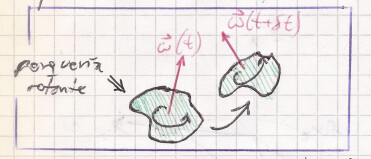
\includegraphics[scale=0.4]{images/fig_mc_rotaciones_porqueria.jpg}

Suponiendo que \vb{U} solo rota 

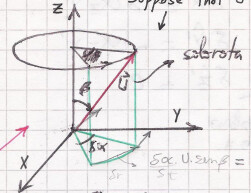
\includegraphics[scale=0.4]{images/fig_mc_rotaciones_u_solorota.jpg}

\[
	\frac{\delta \alpha}{\delta t} U \sin \beta = \Omega U \sin \beta = \vb{\Omega} \times \vb{U}
\]

Un observador rotante vería $dU/dt|_{rot} = 0$ porque no cambian las componentes. Él sería partícipe del movimiento de \vb{U} y 
como la velocidad de rotación de \vb{U} es \vb{\Omega} entonces \vb{U} se ve quieta.

\begin{ejemplo}{\bf Rotación en $\hat{z}$}

Consideremos una rotación en torno a $\hat{z}'$ de manera que como $\delta\hat{z}'=0$ entonces  
$\delta\alpha_x=\delta\alpha_y=0$

Luego, se tienen 
\[
	\delta\hat{x}' = \delta\alpha_z \hat{y}' \qquad \delta\hat{y}' = - \delta\alpha_z \hat{x}'
\]
y entonces debe ser
\[
	\delta \alpha_z \equiv \omega_z . 
\]
\begin{figure}[htb]
	\begin{center}
	\includegraphics[width=0.4\textwidth]{images/fig_mc_rotzej.pdf}	 
	\end{center}
	\caption{}
\end{figure} 

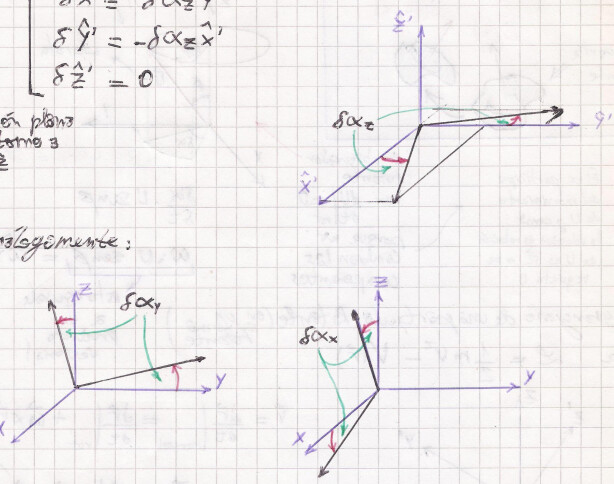
\includegraphics[scale=0.4]{images/fig_mc_rotaciones_ej_rotz.jpg}	 

\notamargen{¿Este gráfico y el anterior son lo mismo?}
\end{ejemplo}


\subsection{Lagrangiano en un sistema rotante}

\[
	\Lag = \frac{1}{2} m v^2 - U(\vb{r})
\]
\[
	\Lag = \frac{1}{2} m ( \vb{v}' + \vb{\Omega} \times \vb{r} )^2 - U(\vb{r})
\]
\[
	\Lag = \frac{1}{2} m \vb{v}'^2 + m \vb{v}' \cdot ( \vb{\Omega} \times \vb{r} ) + 
		\frac{1}{2} m ( \vb{\Omega} \times \vb{r} )^2 - U(\vb{r})
\]
donde esto último es un potencial efectivo $U=U(\vb{r}, \vb{v})$ y para $U$ dependiente de la velocidad
teníamos 
\[
	\vb{F} = -\dpar{U}{q_i} + \frac{d}{dt} \left( \dpar{U}{\dot{q}_i} \right) 
\]

% =================================================================================================
\section{El tensor de inercia}
% =================================================================================================

Siendo $I$ el tensor de inercia buscamos soluciones a
\[
	I \vb{v} = \lambda \vb{v},
\]
o bien en componentes
\be
	 \sum_{j=1}^3 I_{ij} v_j = \lambda v_i
\label{eigen_inercia}	 
\ee
que se trabaja así
\[
	 \sum_{j=1}^3 I_{ij} v_j - \lambda v_i =  \sum_{j=1}^3 ( I_{ij} - \delta_{ij}\lambda ) v_j = 0
\]
lo cual en extenso corresponde al siguiente sistema de tres ecuaciones
\[
	(I_{11} - \lambda)v_1 + I_{12} v_2 + I_{13} v_3 = 0
\]
\[
	I_{21} v_1 + (I_{22} - \lambda) v_2 + I_{23} v_3 = 0
\]
\[
	I_{31} v_1 + I_{32} v_2 + (I_{33} - \lambda) v_3 = 0
\]

Ahora multiplicamos la ecuación \eqref{eigen_inercia} y su conjugada compleja (denotada por $^*$) por $\sum_i v_i$
y $\sum_i v_i^*$, respectivamente, para obtener
\[
	\sum_i v_i \sum_{j=1}^3 I_{ij} v_j^* = \lambda^* \sum_i v_i^*  v_i
\]
\[
	\sum_i v_i^* \sum_{j=1}^3 I_{ij} v_j = \lambda \sum_i v_i v_i^*
\]
Ahora si resto ecuación a ecuación tenemos
\[
	\sum_i \sum_{j=1}^3 ( v_i I_{ij} v_j^* - v_i^* I_{ij} v_j ) =
	(\lambda^* - \lambda )\sum_i v_i^* v_i 
\]
podemos cambiar de índices en el segundo sumando del miembro izquierdo puesto que los índices están sumados y son
por ello mudos ({\it dummies}),
\[
	\sum_i \sum_{j=1}^3 ( v_i I_{ij} v_j^* - v_j^* I_{ji} v_i ) =
	(\lambda^* - \lambda )\sum_i v_i^* v_i 
\]
pero si usamos la propiedad de simetría del tensor de inercia $I_{ij}=I_{ji}$ entonces
\[
	0 = (\lambda^* - \lambda )\sum_i v_i^* v_i 
\]
de modo que como $\vb{v}$ es arbitrario se tiene la importante conclusión de que $\lambda^* = \lambda$.
Los autovalores del tensor de inercia son reales.

Si es por ejemplo $\lambda^s$ uno de los autovalores se pueden despejar
\[
	(v_1^s, v_2^s(v_1), v_3^s(v_1) )\: e^{i\phi}
\]
pero como la fase es la misma para todos me quedo con los módulos (los cuales definirán las direcciones).
Pido 
\[
	{v_1^s}^2 +  {v_2^s(v_1)}^2 + {v_3^s(v_1)}^2 = 1
\]
o dicho de otro modo que la norma sea uno.

Sean $\lambda^p \neq \lambda^s$ entonces 
\[
	\sum_i v_i^p \sum_{j=1}^3 I_{ij} v_j^s = \lambda^s \sum_i v_i^p  v_i^s
\]
\[
	\sum_i v_i^s \sum_{j=1}^3 I_{ij} v_j^p = \lambda^p \sum_i v_i^s v_i^p
\]
y restando ecuación a ecuación y cambiando subíndices como hiciéramos oportunamente,
\[
	\sum_i \sum_{j=1}^3 ( v_i^p I_{ij} v_j^s - v_i^s I_{ij} v_j^p ) =
	(\lambda^s - \lambda^p )\sum_i v_i^p v_i^s 
\]
luego como es nulo el miembro izquierdo resulta que 
\[
	\sum_i v_i^p v_i^s = 0
\]
de modo que son ortogonales $v^p$ y $v^s$. Los autovectores son ortogonales.
\[
	I \vb{v} = \lambda \vb{v} \qquad \longrightarrow \qquad \vb{v}^t I \vb{v} = \vb{v}^t \lambda \vb{v},
\]
pero como la norma de $\vb{v}$ es unitaria, es 
\[
	\vb{v}^t I \vb{v} = \lambda \vb{v}^t  \vb{v} = \lambda
\]
Si armo una matriz $V = ( v^s v^p v^q)$ será en todo su esplendor
\[
	V^t I V = \begin{pmatrix}
	           v_1^s & v_2^s & v_3^s \\
	           v_1^p & v_2^p & v_3^p \\
	           v_1^q & v_2^q & v_3^q
	          \end{pmatrix}
	          I
		\begin{pmatrix}
	           v_1^s & v_1^p & v_1^q  \\
	           v_2^s & v_2^p & v_2^q \\
	           v_3^s & v_3^p & v_3^q
	          \end{pmatrix}
\]
o bien
\[
	V^t I V = \lambda 1
\]
donde entendemos el $1$ como una matriz identidad. Entonces $\lambda^s, \lambda^p, \lambda^q$ son los momentos
principales de inercia
\[
	I = \begin{pmatrix}
	     \lambda^s & 0 & 0 \\
	     0 & \lambda^p & 0 \\
	     0 & 0  &  \lambda^q
	    \end{pmatrix}
\]
Vale que, además,
\[
	\lambda^s = \sum_{ij}  v^s_i I_{ij} v^s_j > 0
\]
puesto que es una forma cuadrática.

Para el objeto debajo de estas líneas rotando en $2\pi/3$ tengo la misma situación física (eje de simetría de
orden tres), entonces tengo eje principal de inercia allí.

La idea es que si pienso en planos siempre se hacen nulos los productos de inercia rotacionales.

Para la siguiente figura el plano de simetría es eje principal, luego es eje principal de inercia.
\begin{figure}[htb]
	\begin{center}
	\includegraphics[width=0.4\textwidth]{images/fig_mc_ejesim.pdf}	 
	\end{center}
	\caption{}
\end{figure} 


% =================================================================================================
\section{Movimiento de un cuerpo asimétrico}
% =================================================================================================

\[
	\vb{L}_{spin} = I \vb{\Omega}
\]
y como la energía se conserva es
\[
	E = T + V
\]
\[
	E = T_{trasl} + T_{rot} + V(R_{cm})
\]
donde cada una se conserva separadamente.

\begin{figure}[htb]
	\begin{center}
	\includegraphics[width=0.4\textwidth]{images/fig_mc_asimbod.pdf}	 
	\end{center}
	\caption{}
\end{figure} 

Usaremos una notación en la cual el subíndice refiere a referido a y el supraíndice a de qué puntos/puntos
\[
	\left.\vb{L}\right|_{0}^{sist} = \left.\vb{L}_{orb}\right|_{0}^{cm} + \left.\vb{L}_{spin}\right|_{cm}^{sist}  
\]
\[
	\left.\frac{d\vb{L}^{orb}}{dt}\right|_{in} = \vb{\tau}_0^{cm} = \vb{R}_{cm} \times \vb{F} =
							\vb{R}_{cm} \times - M g \hat{z} \neq 0
\]
de tal manera que el $\vb{L}^{orb} \equiv \vb{L}_0^{cm}$ no se conserva.

El que se conserva es $\vb{L}^{spin}$ pues pensamos la $\vb{F}=M\vb{g}$ aplicada en el centro de masa que es el origen
y que tiene $\vb{R}_{cm}=0$.
\[
	\vb{L}^{spin} = L_1 \hat{1} + L_2 \hat{2} + L_3 \hat{3} = I_1\Omega_1 \hat{1} + I_2\Omega_2 \hat{2} + I_3\Omega_3 \hat{3}
\]
y podemos escribir
\[
	T_{rot} = \frac{1}{2} \left( I_1\Omega_1^2 + I_2\Omega_2^2 + I_3\Omega_3^2 \right)
\]
\[
	T_{rot} = \frac{L_1^2}{2 I_1} + \frac{L_2^2}{2 I_2} + \frac{L_3^2}{2 I_3}
\]
\[
	1  = \frac{L_1^2}{2 I_1 T_{rot}} + \frac{L_2^2}{2 I_2 T_{rot}} + \frac{L_3^2}{2 I_3 T_{rot}}
\]
\begin{figure}[htb]
	\begin{center}
	\includegraphics[width=0.4\textwidth]{images/fig_mc_asimbod2.pdf}	 
	\end{center}
	\caption{}
\end{figure} 
Entonces, si se da que $I_3 > I_2 > I_1$ se tiene 
\[
	L_{spin}^2 = L_1^2 + L_2^2 + L_3^2 \qquad L^2 =  I_1^2\Omega_1^2 + I_2^2\Omega_2^2 + I_3^2\Omega_3^2
\]
donde como se conservan $T_{rot} \equiv T$ y $L_{spin} \equiv L$ 
\[
	2 T = \frac{L_1^2}{I_1} + \frac{L_2^2}{I_2} + \frac{L_3^2}{I_3} \qquad L^2 = L_1^2 + L_2^2 + L_3^2
\]
de la primera deducimos un elipsoide de semiejes en $L_i$ y de la segunda una esfera de radio $L$ en $L_i$.
\notamargen{Esto está super oscuro. No sé qué se quiso decir, tal vez se halle explicado mejor en la carpeta.}
\begin{figure}[htb]
	\begin{center}
	\includegraphics[width=0.4\textwidth]{images/fig_mc_asimbod3.pdf}	 
	\end{center}
	\caption{}
\end{figure} 
\[
	2 I_3 T > 2 I_2 T > 2 I_1 T
\]
\[
	L^2 > 2 I_3 T	\qquad L_1^2 + L_2^2 + L_3^2 > \frac{I_3}{I_1} L_1^2 + \frac{I_3}{I_2} L_2^2  + L_3^2
\]
\[
	L_1^2 \left( \frac{I_1 - I_3}{I_1} \right) + L_2^2 \left( \frac{I_2 - I_3}{I_1} \right)  > 0
\]
pero esto no vale. Asimismo tampoco vale que 
\[
	L^2 < 2 I_1 T
\]
y resulta 
\[
	2 I_3 T > L^2 > 2 I_1 T
\]
entonces $L_{spin}$ (su punta) se mueve en la intersección de una esfera y un elipsoide.
Estos movimientos son periódicos.

La peonza tiene movimientos estables para la rotación en torno a $\hat{x}_1, \hat{x}_3$ pero inestables en
torno a $\hat{x}_2$. El movimiento puede resolverse mediante ecuaciones de Euler.
Es estable rotar en torno al mayor o menor momento de inercia lo que generará un movimiento oscilatorio
para \vb{\Omega} ($\omega^2 > 0$), en cambio es inestable rotar en torno al momento de inercia intermedio, lo cual generará
un movimiento armónico para \vb{\Omega} ($\omega^2 < 0$).

Con \vb{L} constante si \vb{L }$\parallel$ \vb{\Omega} entonces ambos son constantes (corresponde a una rotación). Se consigue 
con \vb{\Omega} en la dirección del eje principal. Si \vb{L }$\nparallel$ \vb{\Omega} entonces \vb{\Omega} oscila en torno a
\vb{L}.



% \bibliographystyle{CBFT-apa-good}	% (uses file "apa-good.bst")
% \bibliography{CBFT.Referencias} % La base de datos bibliográfica

\end{document}
